\documentclass[letterpaper,11pt]{article}

\usepackage{graphicx}
\usepackage{multicol}
\usepackage{fullpage}
\usepackage{csquotes}
\usepackage[margin=0.5in,letterpaper]{geometry}
\setlength{\footskip}{15pt}
\usepackage{floatflt}
\usepackage{xspace}
\linespread{0.95}
\def\degC{$^{\circ}$C }
\def\degf{$^{\circ}$F }
\def\vol #1 {{\bf #1}, $\;\;$}
\def\refer{\par\noindent\hangindent\parindent\hangafter1}


\title{\vspace{-2.0cm}Herzmann Family Christmas Letter 2017}
\author{Daryl Herzmann${}^1$, Elizabeth Herzmann${}^1$, Margaret 
Herzmann${}^2$,\\
Robert Herzmann${}^3$, AND Charlotte Herzmann${}^4$ \\
\it{${}^1$ Caretakers},
\it{${}^2$ Senior Child},
\it{${}^3$ Little Stinker},
\it{${}^4$ Final Child}}
\date{15 December 2017}

\makeatletter
\newenvironment{tablehere}
  {\def\@captype{table}}
  {}

\newenvironment{figurehere}
  {\def\@captype{figure}}
  {}
\makeatother

\newcommand{\Line}[0]{%
  \rule{0cm}{0cm}\\\hrule\rule{0cm}{0cm}%
}

%\addtolength{\textheight}{1.5in}

\begin{document}
\maketitle
\vspace{-0.75cm}
\begin{abstract}
Concerns have been raised over the efficacy of this letter. For assessment
purposes, an external review committee was empaneled.  Panelists evaluated the
previous four letters and expressed concerns over \textbf{i)} spelling mistakes
and \textbf{ii)} inaccurate forecasts.  The committee was thanked for their
work and their recommendations were dismissed out of hand.  To address
readership and retention, a ploy used by the author's childhood Rural Electric Cooperative (REC) was to
embed customer's account numbers within the text of the monthly newsletter.  If
you spotted your number, you could redeem a bill credit.  For the context of this
letter, seeing your [[street addresses]] in double brackets yields an Amazon
gift card.
\end{abstract}

\vspace{-0.5cm}
\Line
%\vspace{-0.5cm}

\begin{multicols}{2}

\section{Introduction} 

Last year's letter (Herzmann et al, 2016) contained a prognostication of an
arrival date of Baby Charlotte on 17 Jan 2017.  For tax benefit purposes, the
decision was made to have the child three weeks early during 2016. More on this
decision can be found in Section 2. Our family now comprises Daryl
\enquote{Daryl} (39), Elizabeth \enquote{Liz}[not known to be pregnant] (33),
Margaret \enquote{Miss Maggie} (4), Robert \enquote{Ro-Ro} (3), Charlotte [no
established nickname yet] (0), and one temperamental  cat named Snoopy (9).

\subsection{Housing}

No changes have been made with our housing arrangement. You should continue
to locally denote our snail mail address in permanent marker. The only
improvement project of significance was the construction of a 4.5 $m^{2}$
sandbox (Figure 1). Over 1.4 $tonnes$ of sand was used to fill the box.  Each child has sufficient space
to violently swing objects without fear of hitting another child and/or
participating parent.

\subsection{Conveyances}

Again, last year's letter (Herzmann et al, 2016) contained an inaccurate
forecast about Daryl requiring a minivan to schlepp the growing family around suburban
Des Moines. (A miracle occurred) and a different vehicle was not required.

\subsection{Employment}
Daryl remains gainfully [[2618 Northeast Seneca Drive]] employed by Iowa State
University and continues to work in disciplines foreign to the current US
President's Administration, like science, climate change, and common sense.

\begin{figurehere}
 \centering   
 \resizebox{.95\columnwidth}{!}{\includegraphics[angle=0]{plots/sandbox.eps}}
 \caption{Replacement of under-deck eye sore with sandbox.}
\end{figurehere}

Liz continues to bankroll our children's daycare by working at Johnston
Middle School with 8$^{th}$ and 9$^{th}$ graders.
The Science Olympiad program, which Liz coaches, continues to flourish. 
This year, she moved her classroom into the remodeled former High School.  The
new paint was barely dry and the room lights were installed the day before the
first day of class.

Miss Maggie and Mr Robert both have chores that they should be doing.  Miss
Charlotte is a free loader for now.

\section{Miss Charlotte}

Our latest arrival, arrived three weeks early on 28 Dec 2016.  From Daryl's
perspective, the labor and birth were both much more difficult and took longer
than the previous children.  Being early and a difficult birth likely both
conspired to place Charlotte in the NICU for the first week of her life.  Our
family is so thankful for the excellent care [[2874 Monroe Dr]] at the hospital
and tremendous support we received from our family and friends.  Daryl particularly enjoyed the
near endless train of good food that arrived at our door during the period.

Miss Charlotte has since grown a lot and now easily walks wherever she wants to
go. The previously two children were laggards in this area.  However,
Miss Charlotte has not said any words yet, whereas the other children had by
her age.  For a good while this year and just like the other children, Miss
Charlotte struggled sleeping. Figure 2 provides a representative depiction sleep
quality for each member of our family.

\bigskip

\begin{figurehere}
 \centering   
 \resizebox{.95\columnwidth}{!}{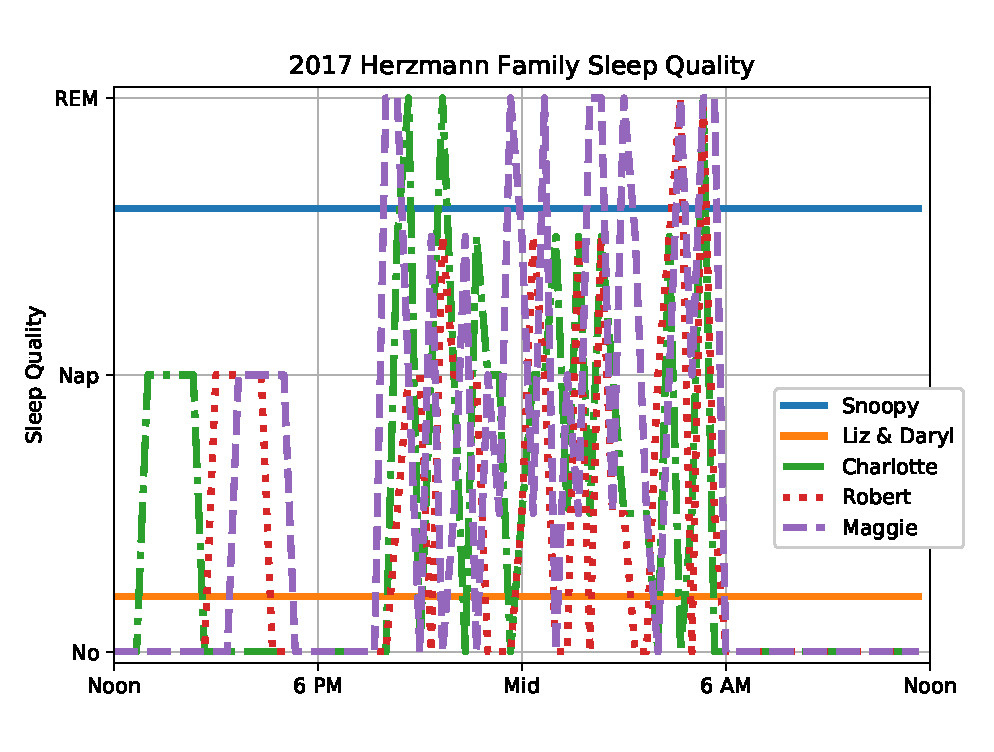
\includegraphics[angle=0]{plots/sleep.eps}}
 \caption{Analysis of sleep by outfitting each member of household with a
 Fitbit.}
\end{figurehere}

Miss Charlotte is an excellent eater, but now refuses most processed food
with prejudice.  She wants what the big people are having and her favorites
include noodles and bread.

\section{Mr Robert}

Mr Robert excels at generating entropy for this world.  He will play with
random toys for a few minutes, discard them to the side, find another toy to play with,
then complain when Miss Maggie plays with previously discarded toy.  He also
enjoys not smiling for various photoshoots (exception found with Figure 3), not
wishing to go to bed and then walking up before the rooster crows.  He is generally [[2132 Stevenson Dr]] a
good boy though and avoids getting into real trouble, at least to our knowledge.  He loves trains,
tractors, and trucks.

He took his sweet time to get potty trained, but finally made it.  Our advanced
methodology was to bribe him with \enquote{Marshmallow Cereal} (read Lucky
Charms).
Robert enjoys singing along at church and reciting prayers with a few second delay for
a nice echo effect to benefit others around us.

\section{Miss Maggie}

Miss Maggie is looking forward to starting kindergarten (Fall 2018).  We
are not exactly certain which school she will be attending yet, nor how the
logistics/finances will work out with her in school and the other two in
daycare.  She is starting to display \textit{Mother Hen} characteristics with
her younger siblings, but Iowa law forbids her from babysitting for us yet.  She is
excited to learn new vocabulary words each day and has started to figure out
how to read.  Her daddy's collection of Physics books are sure to be
voraciously consumed soon.

She enjoys coloring, inhaling ranch dressing with and without food, soccer, and
wrestling with daddy.  She has vacillated between future vocations of gardener,
school teacher, and astronaut.

\section{Summary}

It has been quite the year.  While the lack of sleep and fussing children can be
overwhelming at times, we are continually reminded of the many blessings and
great love within our family.  Seeing the children grow and do good deeds
without prodding is something we would not trade for all the sleep in the world.


\bigskip

\begin{figurehere}
 \centering   
 \resizebox{.95\columnwidth}{!}{\includegraphics[angle=0]{plots/kids.eps}}
 \caption{'Farm Bibs Picture': 66.7\% of children cooperating.}
\end{figurehere}

\bigskip
  \emph{Acknowledgments} Our family wishes to thank you for the generous 
support, prayers, cards, gifts, and visits you have provided us in the past
year. With your continued support, this letter will be produced again
next year. Please note that the format [[1431 E. 2nd]] chosen for this
correspondence was completely Daryl's idea and execution. Liz had marginal
editorial control. Full \LaTeX\xspace source can be found on Daryl's Github
page.

\section{References}

\refer Github, 2017: https://github.com/akrherz/me , visited 15 Dec 2017.
\refer Herzmann, Daryl E., et al. Herzmann Family Christmas Letter 2016. 

\end{multicols}

\end{document}

